\part{L'humain se concentre sur les tâches qui nécéssite d'avoir des traits humains}
\chapter{l'Intelligence Artificelle ne peux pas remplacer l'humain pour toutes les tâches}
\section{Intelligence Artificielle Forte}
L'intelligence artificelle forte est l'intelligence
telle qu'elle existe chez l'homme, une somme de procédés cognitifs avancés mais
même aujourd'hui le fonctionnement du cerveau et de l'intelligence reste mystérieuse
et donc la faisabilité d'une IA forte est sans cesse remise en question.

\subsection{Prérequis}
puisque la définition de l'Intelligence elle même reste flou, il est difficile 
de donner une liste exacte et correcte des critères pour qu'une IA forte 
puisse exprimer une intelligence semblable à celle de l'homme mais 
il une liste de critères semble être indéniablement nécéssaires pour remplir 
les critères et la majorité des chercheurs en intelligence artificelle semble 
s'être mis d'accord sur la liste de critères suivantes: \newline

%TODO approfondir chaque item
\begin{itemize}
    \item Capacité de raisonnement et de jugement: 
    \begin{quotation}
    <<tel que défini sur wikipedia: "Le raisonnement est un processus cognitif permettant 
    de poser un problème de manière réfléchie en vue d'obtenir un ou plusieurs résultats. 
    L'objectif d'un raisonnement est de mieux cerner (comprendre) un fait ou d'en vérifier la réalité, 
    en faisant appel alternativement à différentes « lois » et à des expériences, 
    ceci quel que soit le domaine d'application : mathématiques, système judiciaire, 
    physique, pédagogie, etc.>>
    \footnote{\url{https://fr.wikipedia.org/wiki/Raisonnement}}  
    \end{quotation}

    c'est en somme la capacité à trouver de manière générique la solution à un problème appliqué 
    ou abstrait associé à la capacité à utiliser les connaissances nécéssaires pour pouvoir
    résoudre ledit problème. 
    \newline

    \item Capacité à conceptualiser ses connaissances: \newline
    Il s'agit d'avoir une IA capable de vider tout "contenu" d'une connaissance et d'en garder 
    que l'idée abstraite, la concptualisation des connaissances est essentielle dans l'apprentissage
    et un des principes qui explique le fossé qui sépare le cerveau humain de l'intelligence 
    artificelle faible. %TODO peux encore ameliorer cet item
    \newline
    

    \item Capacité de communication dans un langage naturel: \newline
    La capacité à parler une langue humaine de manière fluide 
    tout en comprenant les spécificité du langage mais aussi la sémantique du langage,
    la communication dans un langage naturel est souvent associée à l'intelligence humaine 
    et principalement utilisé pour mesurer l'intelligence (test de turing par exemple)
    à cause des processus nécéssaires tel que la représentation mentale, l'empathie, 
    la métacognition. 
    \newline
    

    \item Capacité de planification:
    %TODO indiquer 
    \begin{quotation}
        <<En intelligence artificielle, la planification automatique 
    (automated planning en anglais) ou plus simplement planification, vise à développer des 
    algorithmes pour produire des plans typiquement pour l'exécution par un robot ou tout autre agent.
    Les logiciels de planification qui incorporent ces algorithmes s'appellent des planificateurs. 
    La difficulté du problème de planification dépend des hypothèses de simplification qu'on tient 
    pour acquis, par exemple un temps atomique, un temps déterministe, une observabilité complète, etc.>>
    \footnote{\url{https://fr.wikipedia.org/wiki/Planification_(intelligence_artificielle)}} 
    \end{quotation}
        
    La planification automatique se base sur 3 paramètres d'entrée: 
    \begin{itemize}
        \item état de départ
        \item actions possibles 
        \item objectif \newline
    \end{itemize}

    \begin{figure}[!h]
        \centering
        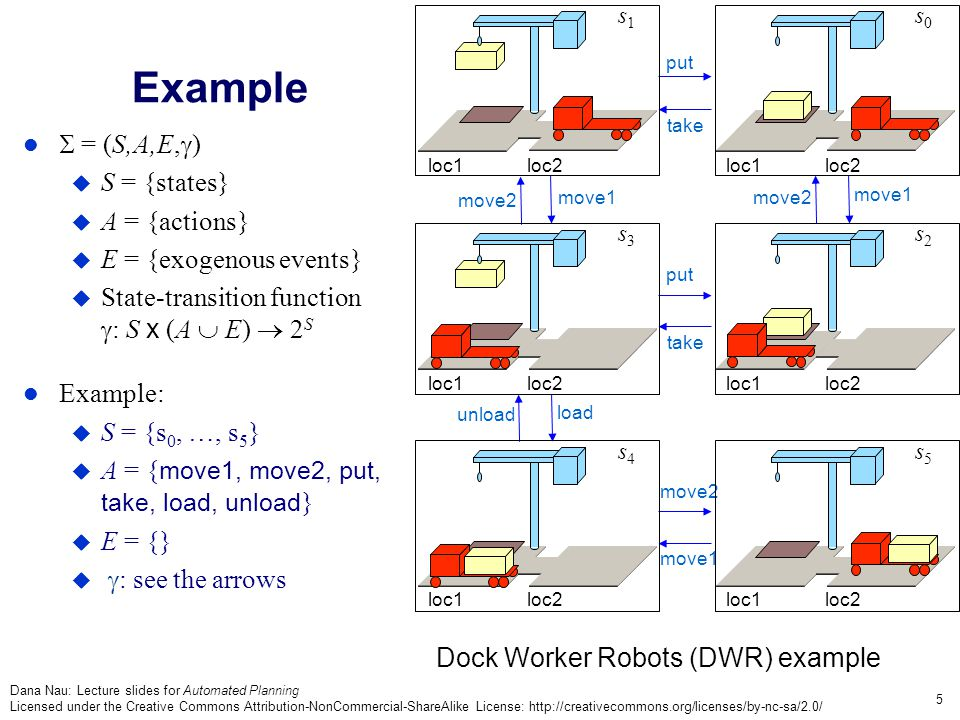
\includegraphics[width=0.7\textwidth]{Images/automatedPlanification}
        \caption{Planification automatique avec un automate}
        \label{fig:chineseroom}
    \end{figure}
    
    la difficulté de la planification automatique avec une intelligence artificelle forte est dù
    au charactère non-déterministe de la majorité des actions que cette dernière doit réaliser,
    contrairement à un automate ou toutes ses actions sont déterministes, de plus 
    la liste des actions possible n'est plus réellement fixe. \newline

    

\end{itemize}


\subsection{Freins majeur de la création d'Intelligence Artificelle Forte}
%la meta cognition est un des freins majeur (la cognition sur la cognition)

%le cheminement de pensee de cette partie est d'expliquer cette experience 
%pour montrer qu'une IA ne peu pas actuellement etre intelligente comme un humain
%et utiliser la conclusion de cette section sur lequel ce basera pour 
%eliminer la possibilité de remplacement de l'humain dans le futur proche 
%dans les métiers qui necessitent de l'intelligence humaine
%
%un contre argument en particulier de cette experience peut etre partiellement 
%invalidé: celui de Douglas Hofstadter qui dit que les règles syntaxiques à 
%elle seule ne suffisent pas à elle seule pour reproduire la 
%compréhension du langage il faut comprendre le monde 
%
%mon contre argument est justement d'associer le manuel utilisé dans la piece fermé
%associé à un algorithme de deep learning entrainé sur des millions de data de 
%conversation, pour avoir la partie syntaxique (homme+manuel) 
%et la partie sémantique (deep learning)
%
%en soit le deep learning en lui meme invalide le contre argument
%exemple: personnal assistants etc mais seulement dans des cas très précis
%puisque les assistant ne passerait pas le test de turing 
\newpage
\section{L'experience de pensée "Chinese Room"}
En 1980 John Searle, philosophe américain, publie son article "Minds, Brains, and Programs" dans la revue 
scientifique "Behavioral and Brain Sciences" qui donna lieu à de grands débat dans le domaine philosophique 
mais surtout dans le domaine de l'intelligence artificelle, 
la source de ces débats est une expérience de pensée qui se nomme "Chinese Room". \newline

\begin{figure}[!h]
    \centering
    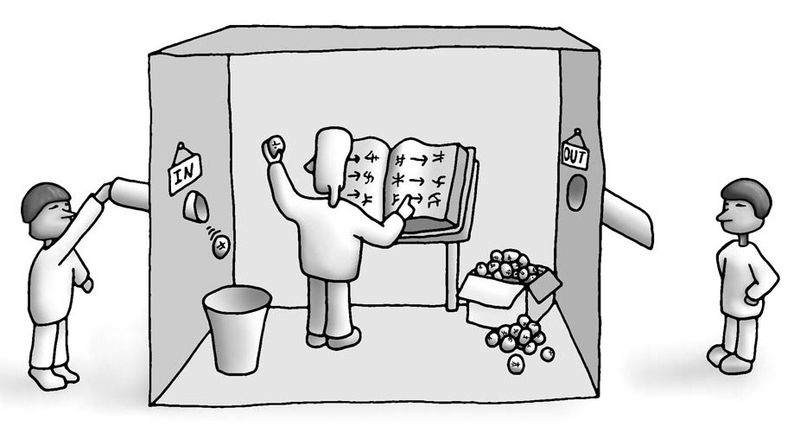
\includegraphics[width=0.8\textwidth]{Images/chineseroom}
    \caption{Chinese room experiment - wikicommons}
	\label{fig:chineseroom}
\end{figure}

Cette expérience est définie comme suit: \newline
il y a, enfermé dans une piece sans aucun moyen de contact vers l'exterieur, une personne anglophone qui ne comprend 
pas le chinois et dans cette piece des boites remplies de symboles chinois ainsi qu'un manuel d'instructions.
Cette personne reçois des symboles chinois envoyé par une personne parlant chinois qui sont en réalité des questions,
dans le manuel d'instruction est indiqué quoi renvoyer en fonction de ce que la personne anglophone reçois,
la personne renvoie des symboles qui sont des réponses à la question reçue, la personne parlant le chinois
pense ainsi parler à une personne qui connaît la langue alors que ce n'est pas le cas. \newline 

l'argument de cette expérience est que meme si la machine répond aux questions qui semble laisser penser 
la présence de capacité à penser (une IA forte) elle ne fait en réalité que manipuler des symboles 
sans les interpreter (IA faible). \newline

l'objectif de cette experience est d'invalider la capacité du test du turing à établir si une 
intelligence artificelle a la capacité de penser, le test de turing est une expérience à l'aveugle 
ou une personne converse avec un interlocuteur qui est est soit une vrai personne ou un humain 
si le sujet avec qui l'IA converse n'est pas capable de detecter qu'il ne parle pas avec un humain mais
une machine cette dernière réussie le test or l'experience chinese room essaie de démonter 
justement que la capacité à converser ne va pas forcément prouver l'intelligence et la capacité à penser  
car il suffit de manipuler les symboles d'une manière assez complexe pour tromper l'interlocuteur humain.

% John Searle n'essaie pas de montrer qu'il n'est pas possible d'avoir une IA forte mais qu'avec 
% les ordinateurs et supercalculateurs conventionnels actuellement utilisés elle n'est pas encore 
% à notre portée. 


%explication en profondeur de la chinese room

%une ia entoure des symboles de metadonnée pour ensuite "passer cela dans une fonction et donner un
%résultat, dans le cas d'un humain les symboles, la langue n'est que l'incarnation 
%physique d'un objet/processus mental: les lettres à elles seules ne veulent rien 
%dire, les langages eux meme ne veulent rien dire, leur utilité réside seulement 
%dans le sens qu'on leur donne, or les machine et l'IA d'aujourdhui ou des prochaines années
%ne fonctionne que de maniere concrete 

%notre vision n'est pas seulement patterne matching comme les AI de reconnaissance d'image 
\subsection{Simuler l'intelligence n'est pas suffisant pour créer l'intelligence émotionnelle}

%montrer que l'IA ne peut pas avoir de conscience et donc la meme intelligence que l'humain, 
%ce qui veut dire que l'humain ne pourra être remplacé que dans les taches non repetitives 

%ce qui suit sont des notes de reflexion sans aucun sens 
% lhomme apprend à la machien = on injecte en quelquesorte la projection de notre conscience 
%on utilise la langue pour communiquer ce que l'on veut or notre langue = sementique => "syntax does not 
%suffice for semantic"  
%
%compiler = grammar rule + regle semantic écrite à la main => une infinité de regles pour l'esprit en plus 
%du bon sens commun 

%le livre est écrit par un humain, et l'anglais n'est qu'un intermediaire => l'ecrivain du livre aka 
%programmeur doit savoir parler chinois = est ce l'on parle au programmeur au final ? 

%And the reason is that 
%the entire system, me, symbols, rule books, room, etc., contain only Chinese symbolic devices but no meanings
%le langage par lui meme est symbolique et n'est qu'un support physique du meaning qu´on leur donne




\subsection{Application à la problématique de l'automatisation des métiers}